\documentclass[11pt,a4paper]{article}
 
\newcommand{\tumsoTime}{13:00 น. - 16:00 น.}
\newcommand{\tumsoRound}{2}
 
\usepackage{../tumso}
 \usepackage{tikz}
 
\begin{document}
 
\begin{problem}{ก้อน ๆ}{}{}{1 second}{256 megabytes}{100}

มี simple graph (graph ที่ไม่มี self-loop หรือ multiple edge) ขนาด $n$ vertices $m$ edges ให้หาว่ามี "ก้อน" อยู่กี่ "ก้อน"

ให้นิยาม "ก้อน" ใน graph หนึ่งว่าเป็นกลุ่มของ vertices ที่อยู่ใน cycle เดียวกัน หากมีหลาย cycle ใช้ vertices อันใดอันหนึ่งร่วมกัน ให้นับว่า vertices ในทุก cycle เหล่านั้นอยู่ใน "ก้อน" เดียวกัน

หากมี vertices ที่ไม่ได้เป็นส่วนหนึ่งของ cycle ใดเลย ให้ถือว่า vertex นั้นเป็น "ก้อน" ที่มีสมาชิกเพียง $1$ ตัว

หมายเหตุ : cycle หรือ วังวน คือกลุ่มของ vertices ที่มีเส้นเชื่อมเรียงกันเป็นวง สมาชิกทุกตัวในนั้นสามารถเดินวนกลับมาหาจุดเริ่มต้นที่เดิมได้โดยไม่ผ่าน vertices ซ้ำเดิม

เช่น

 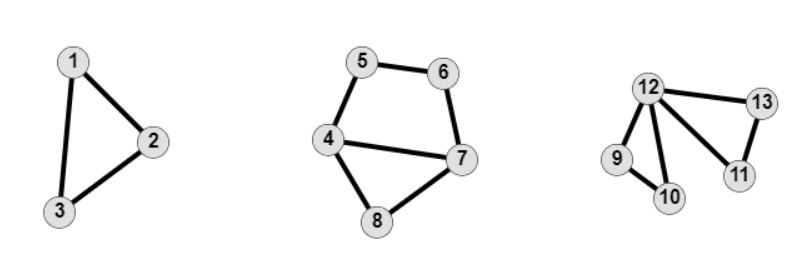
\includegraphics[width=\textwidth]{09-chunk-in-graph/1.jpg}

ทั้งสามรูปนี้นับว่าแต่ละรูปประกอบด้วย $1$ "ก้อน"

และ 

 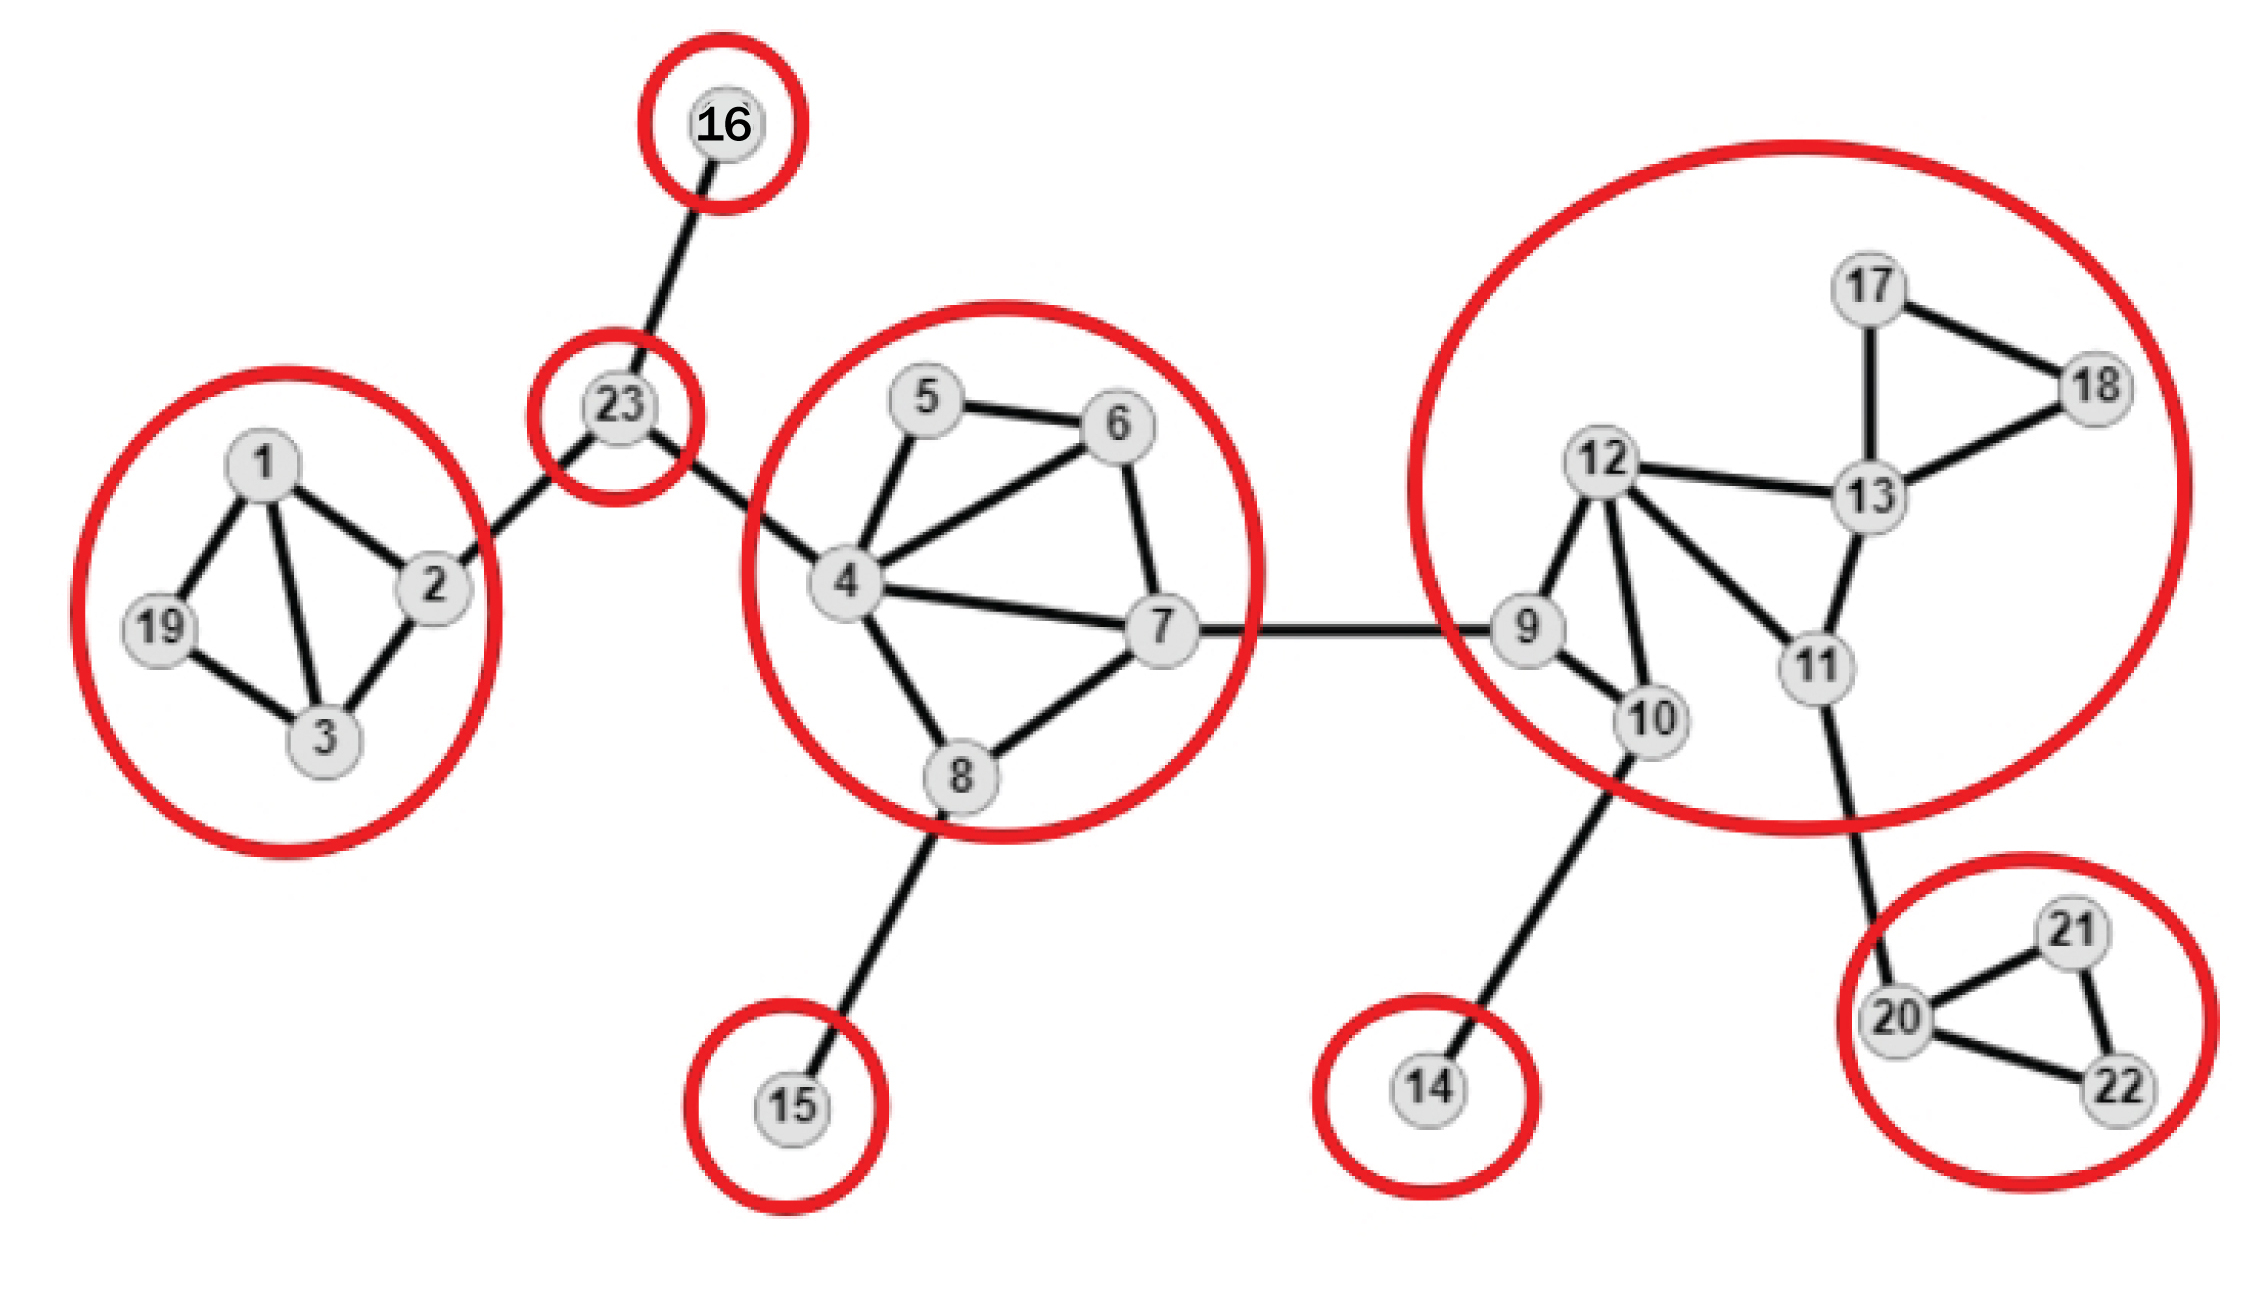
\includegraphics[width=\textwidth]{09-chunk-in-graph/2.jpg}

ในรูปนี้มี "ก้อน" จำนวน $8$ ก้อน ตามวงกลมสีแดงที่วงไว้

\InputFile

บรรทัดแรก ระบุจำนวนเต็ม $n$ และ $m$ $(1 \leq n \leq 5\cdot 10^5 , 0 \leq m \leq min(\frac{n(n-1)}{2}, 10^6))$ โดยที่ $n$ แทนจำนวน vertices และ $m$ แทนจำนวนเส้นเชื่อม 

บรรทัดที่ $1+i$ แต่ละบรรทัดระบุจำนวนเต็ม $2$ ตัว ระบุ $p$ และ $q$ $(1 \leq p,q \leq n)$ ตามลำดับโดยที่ $p$ และ $q$ แทนเส้นเชื่อมเส้นที่ $i$ ที่เชื่อมระหว่าง vertex $p$ กับ $q$ $(1 \leq i \leq m)$

\OutputFile

บรรทัดเดียว แสดงจำนวน "ก้อน" ในกราฟนี้

\Scoring
ชุดทดสอบจะถูกแบ่งเป็น 3 ชุด จะได้คะแนนในแต่ละชุดก็ต่อเมื่อโปรแกรมให้ผลลัพธ์ถูกต้องในชุดทดสอบย่อยทั้งหมด
 
\begin{description}
\item[ชุดที่ 1 (15 คะแนน)] $n \leq 30$
\item[ชุดที่ 2 (31 คะแนน)] $n \leq 1000$
\item[ชุดที่ 3 (54 คะแนน)] ไม่มีเงื่อนไขเพิ่มเติม
\end{description}

\Examples

\begin{example}
\exmp{23 31
1 2
2 3
1 3
19 1
19 3
2 23
23 24
23 4
4 5
5 6
4 6
4 7
6 7
4 8
7 8
8 15
7 9
9 10
9 12
10 12
10 14
12 11
11 13
12 13
13 17
13 18
17 18
11 20
20 21
21 22
20 22
}{9
}%
\end{example}
 
\end{problem}
 
\end{document}